%!TEX root = ../paper.tex
This section discusses the results presented in \cref{s:results}. We consider the lack of difference in performance between the estimators in \cref{s:discussion:performance}. The next section discusses the anisotropy of the kernels used by the shape-adaptive estimators. 

\subsection{Performance}
\label{s:discussion:performance}
%!TEX root = ../paper.tex

% Hardly any difference between estimators
One of the most striking observations from \cref{s:results} is that the difference in performance between the two estimators is minimal. 
	
	% Study differences further mbe vs sambe plot
		% Single Sphere Sets
		Plotting the densities estimated by \sambe as a function of those estimated by \mbe shows no interesting differences between the two estimators for data set \ferdosiOne through \baakmanFive. 
		% Multi Sphere Sets
		However for data set \ferdosiTwo through \baakmanThree these plots reveal some differences between the estimators. As can be seen in \cref{fig:discussion:performance:two:mbevssambe}, using shape-adaptive kernels results in estimated densities that are generally higher than those estimated with a fixed-shape kernel for data set \ferdosiTwo and \baakmanTwo. Reviewing the raw data shows that \sambe underestimates densities less than \mbe on points near the mean of `Trivariate Gaussian 1'. The kernels in this neighborhood are all slightly anisotropic, which has allowed the shape-adaptive estimator to use more data points, to better approximate the local densities. Thus showing that estimating densities with shape-adaptive kernels can be advantageous.
		%
		\begin{figure}
			\centering
			\begin{subfigure}{0.3\textwidth}
				\centering
				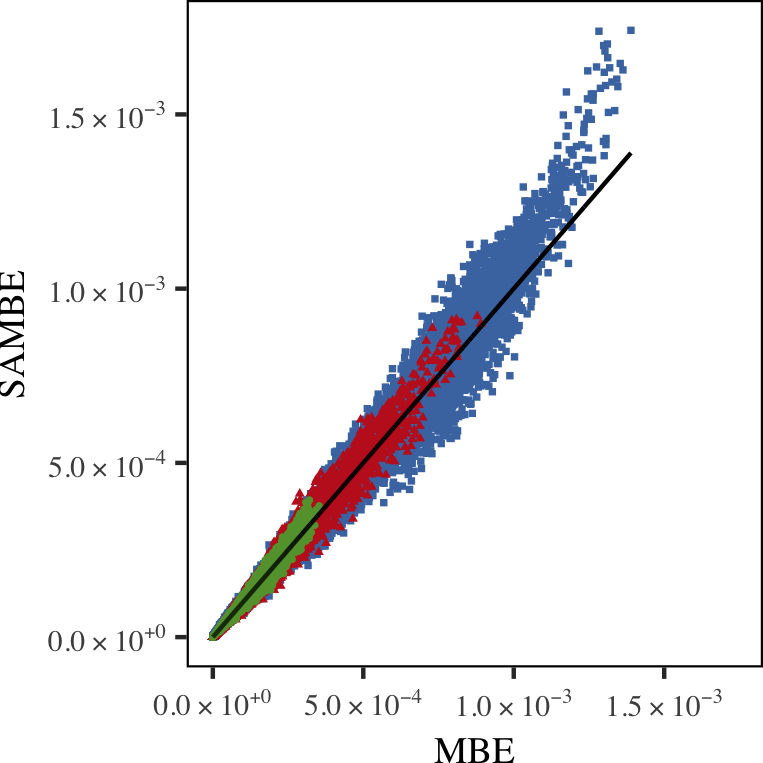
\includegraphics[keepaspectratio=true, width=\textwidth, height=0.23\textheight]{discussion/img/ferdosi_2_60000_mbe_sambe.png}
				\caption{Data set \ferdosiTwo}
				\label{fig:discussion:performance:mbevssambe:ferdosi2}
			\end{subfigure}
			\subfigvspace
			\begin{subfigure}{0.3\textwidth}
				\centering
				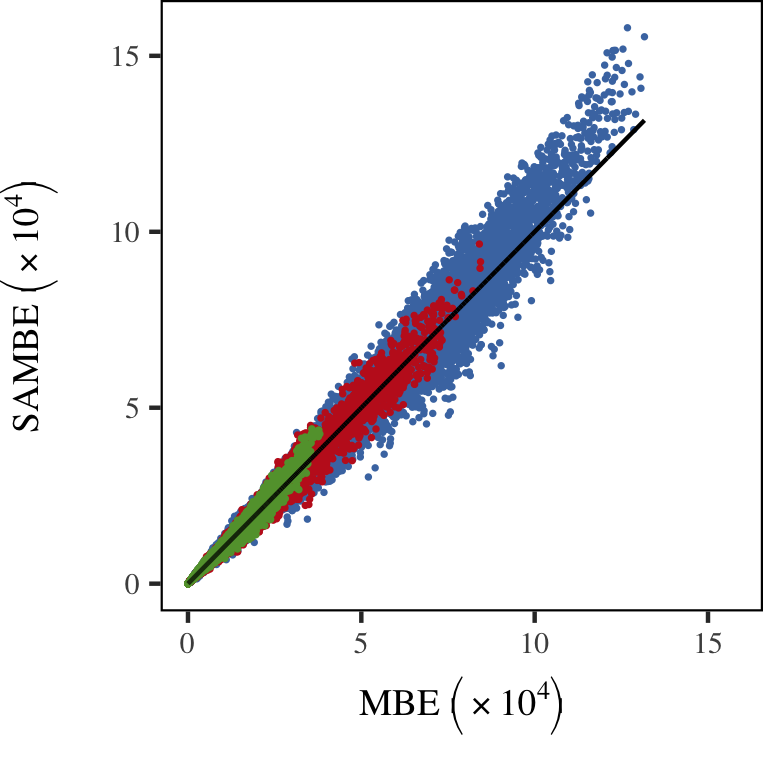
\includegraphics[keepaspectratio=true, width=\textwidth, height=0.23\textheight]{discussion/img/baakman_2_60000_mbe_sambe.png}
				\caption{Data set \baakmanTwo}
				\label{fig:discussion:performance:mbevssambe:baakman2}
			\end{subfigure}	
			\caption{Plots of the densities estimated by \sambe as a function of those estimated by \mbe for data set %
				\subref{fig:discussion:performance:mbevssambe:ferdosi2} % 
				\ferdosiTwo and %
				\subref{fig:discussion:performance:mbevssambe:baakman2} %
				\baakmanTwo.
			}
			\label{fig:discussion:performance:two:mbevssambe}
		\end{figure}
		
		% Ferdosi 3 / Baakman 3
		\Cref{fig:discussion:performance:four:mbevssambe} shows the opposite effect; the densities estimated by \sambe for data set \ferdosiThree and \baakmanThree are generally lower than those estimated by \mbe. Reviewing the raw data shows that the points where the differences in estimated densities between the two estimators are largest lie near the mean of the `Trivariate Gaussian 3' in both data set \ferdosiThree and \baakmanThree. The number of points used in the density estimate by \sambe is consistently lower than the number of points used by the fixed-shape estimator. Given the relatively high anisotropy of the kernels in that area we expect that this is due to the kernels reflecting fine local structures, instead of the global neighborhood. 
		%	
		\begin{figure}
			\centering
			\begin{subfigure}{0.3\textwidth}
				\centering
				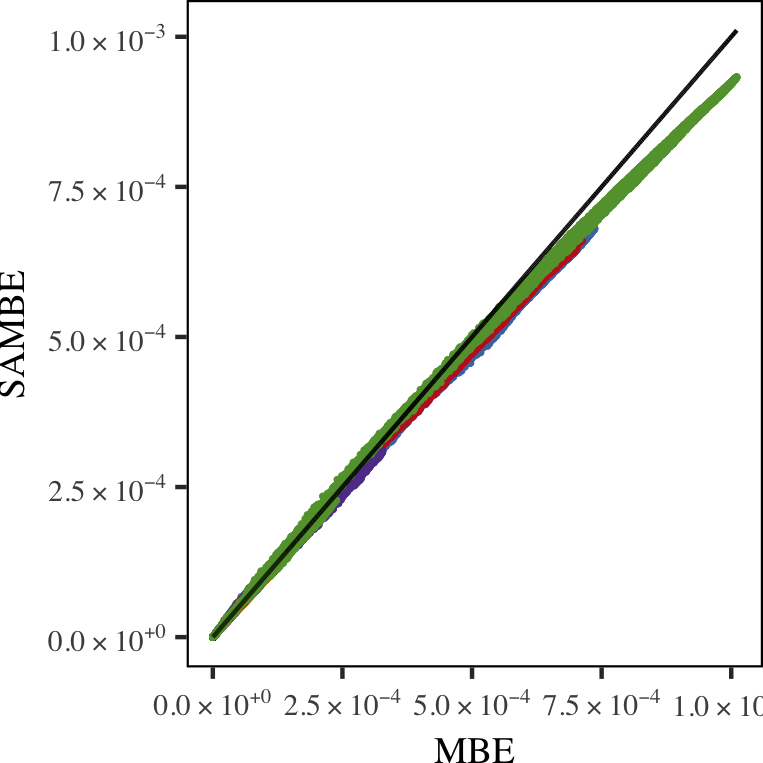
\includegraphics[keepaspectratio=true, width=\textwidth, height=0.23\textheight]{discussion/img/ferdosi_3_120000_mbe_sambe.png}
				\caption{Data set \ferdosiThree}
				\label{fig:discussion:performance:mbevssambe:ferdosi3}
			\end{subfigure}
			\subfigvspace
			\begin{subfigure}{0.3\textwidth}
				\centering
				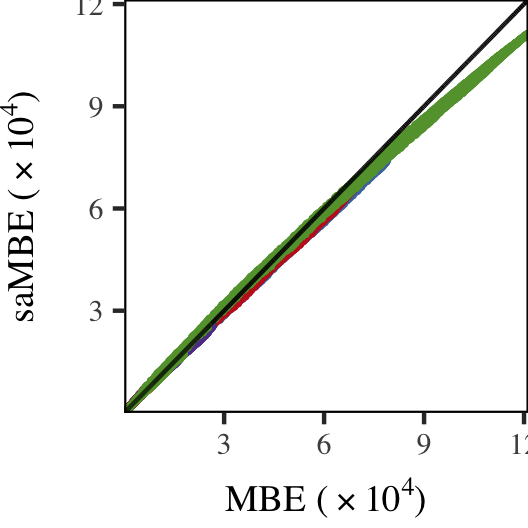
\includegraphics[keepaspectratio=true, width=\textwidth, height=0.23\textheight]{discussion/img/baakman_3_120000_mbe_sambe.png}
				\caption{Data set \baakmanThree}
				\label{fig:discussion:performance:mbevssambe:baakman3}
			\end{subfigure}	
			\caption{Plots of the density estimated by \sambe as a function of those estimated by \mbe for data set %
				\subref{fig:discussion:performance:mbevssambe:ferdosi3} % 
				\ferdosiThree and %
				\subref{fig:discussion:performance:mbevssambe:baakman3} %
				\baakmanThree.
			}
			\label{fig:discussion:performance:four:mbevssambe}
		\end{figure}

	% Where are the differences largest -> plots
	% Single Sphere
		\begin{figure}
			\centering
			\begin{subfigure}{0.23\textwidth}
				\centering
				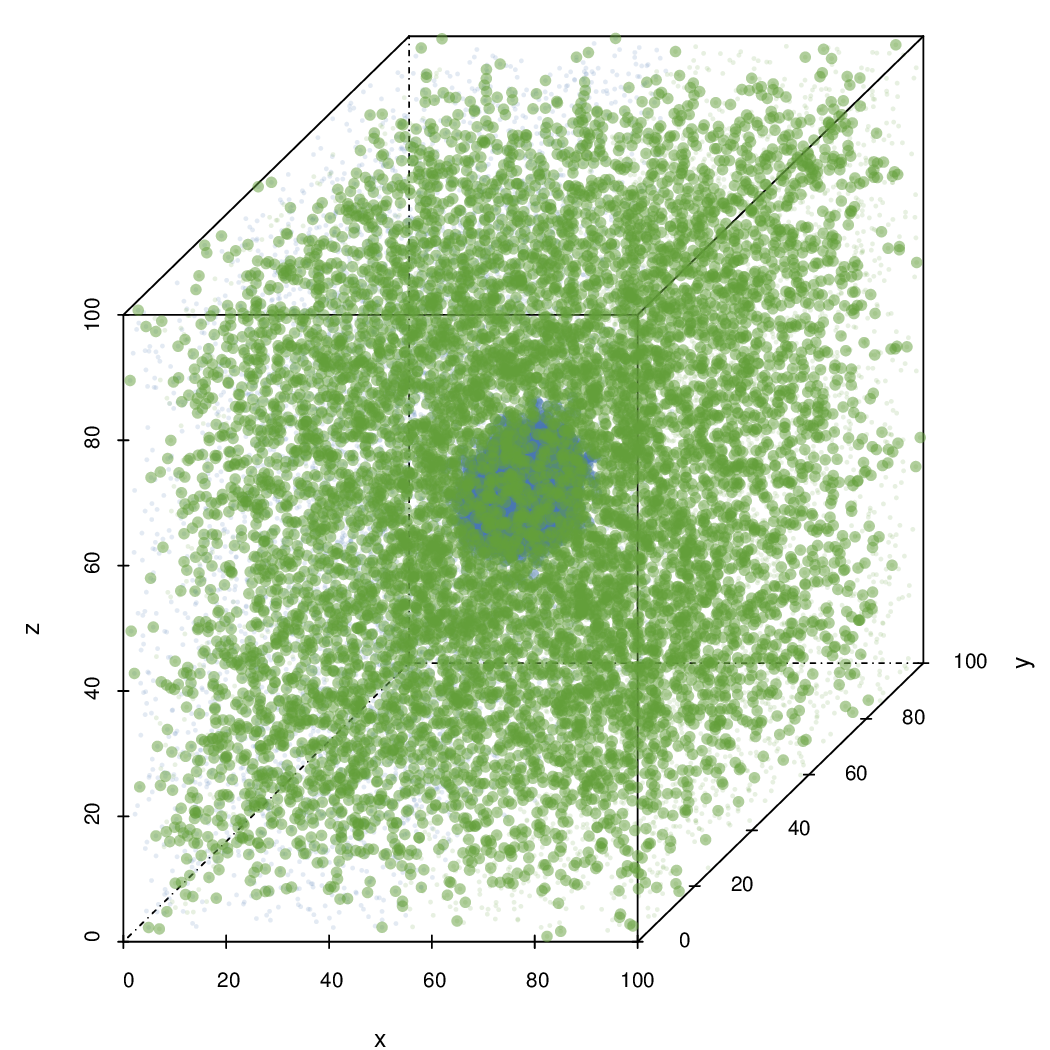
\includegraphics[keepaspectratio=true, width=\textwidth, height=0.23\textheight]{discussion/img/ferdosi_1_abs_error_mbeSmallerThansambe}
				\caption{Data set \ferdosiOne}
				\label{fig:discussion:performance:mbeLowerError:ferdosi1}
			\end{subfigure}
			\begin{subfigure}{0.23\textwidth}
				\centering
				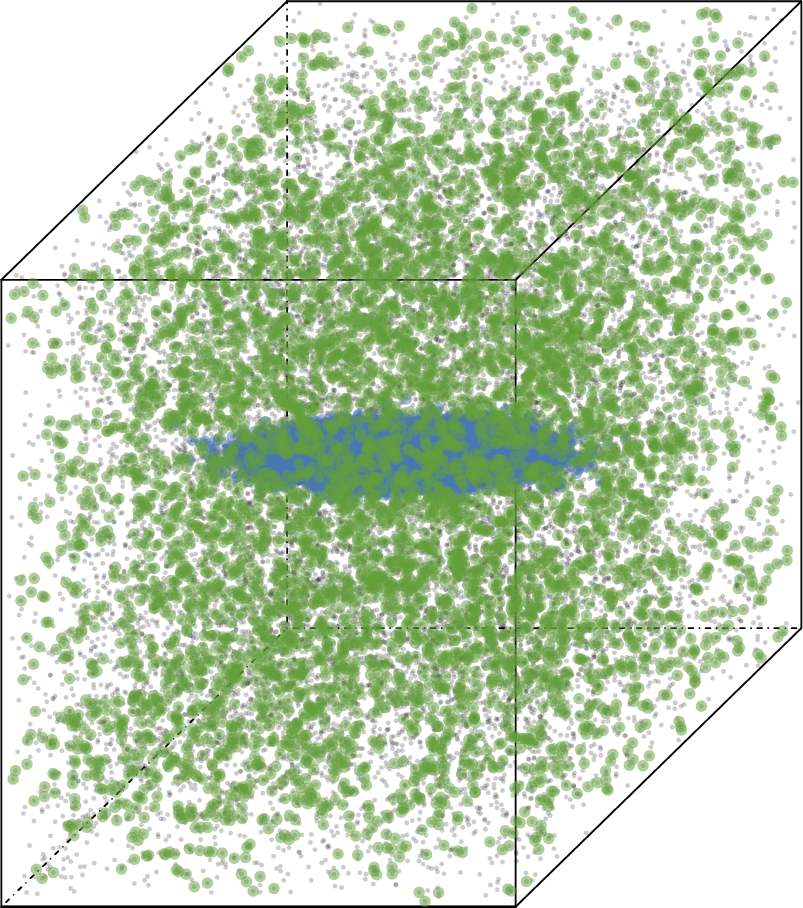
\includegraphics[keepaspectratio=true, width=\textwidth, height=0.23\textheight]{discussion/img/baakman_1_abs_error_mbeSmallerThansambe}
				\caption{Data set \baakmanOne}
				\label{fig:discussion:performance:mbeLowerError:baakman1}
			\end{subfigure}	
			\subfigvspace
			\begin{subfigure}{0.23\textwidth}
				\centering
				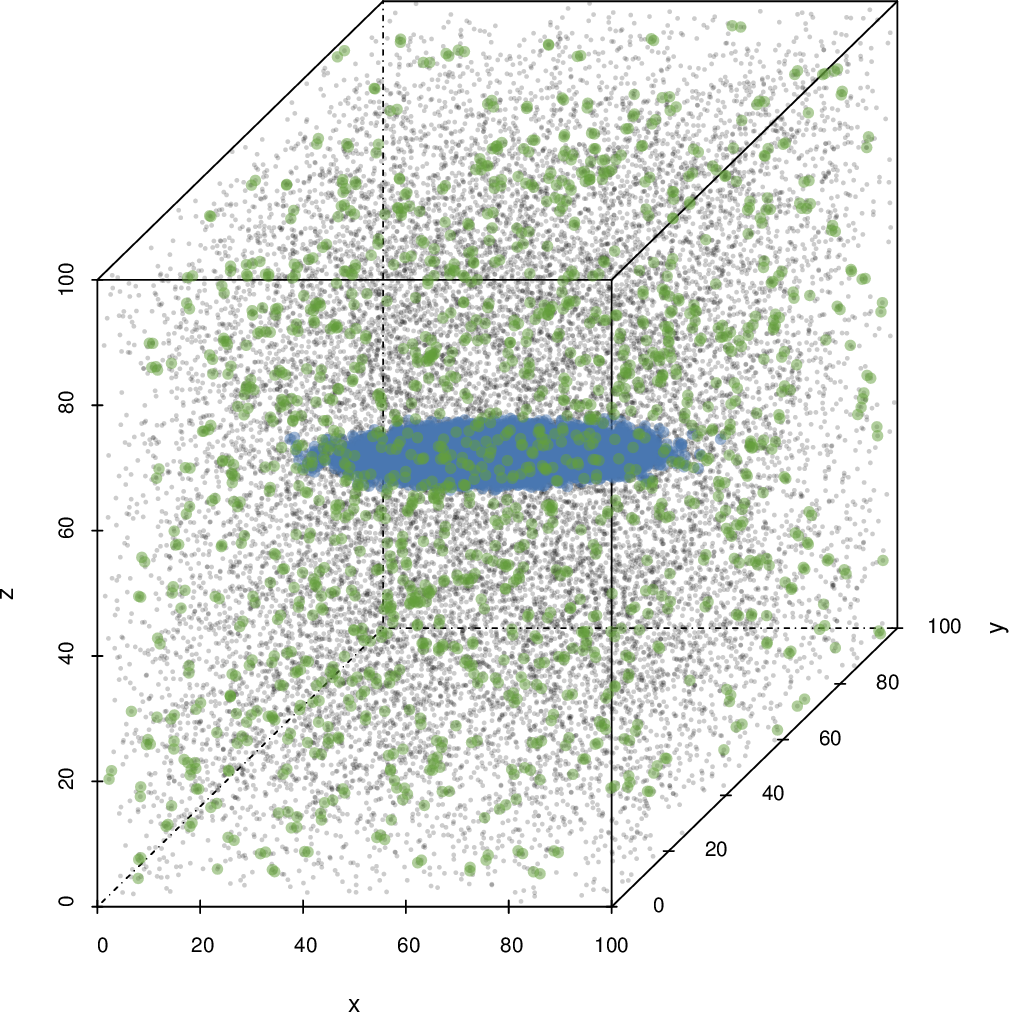
\includegraphics[keepaspectratio=true, width=\textwidth, height=0.23\textheight]{discussion/img/baakman_4_abs_error_mbeSmallerThansambe}
				\caption{Data set \baakmanFour}
				\label{fig:discussion:performance:mbeLowerError:baakman4}
			\end{subfigure}		
			\begin{subfigure}{0.23\textwidth}
				\centering
				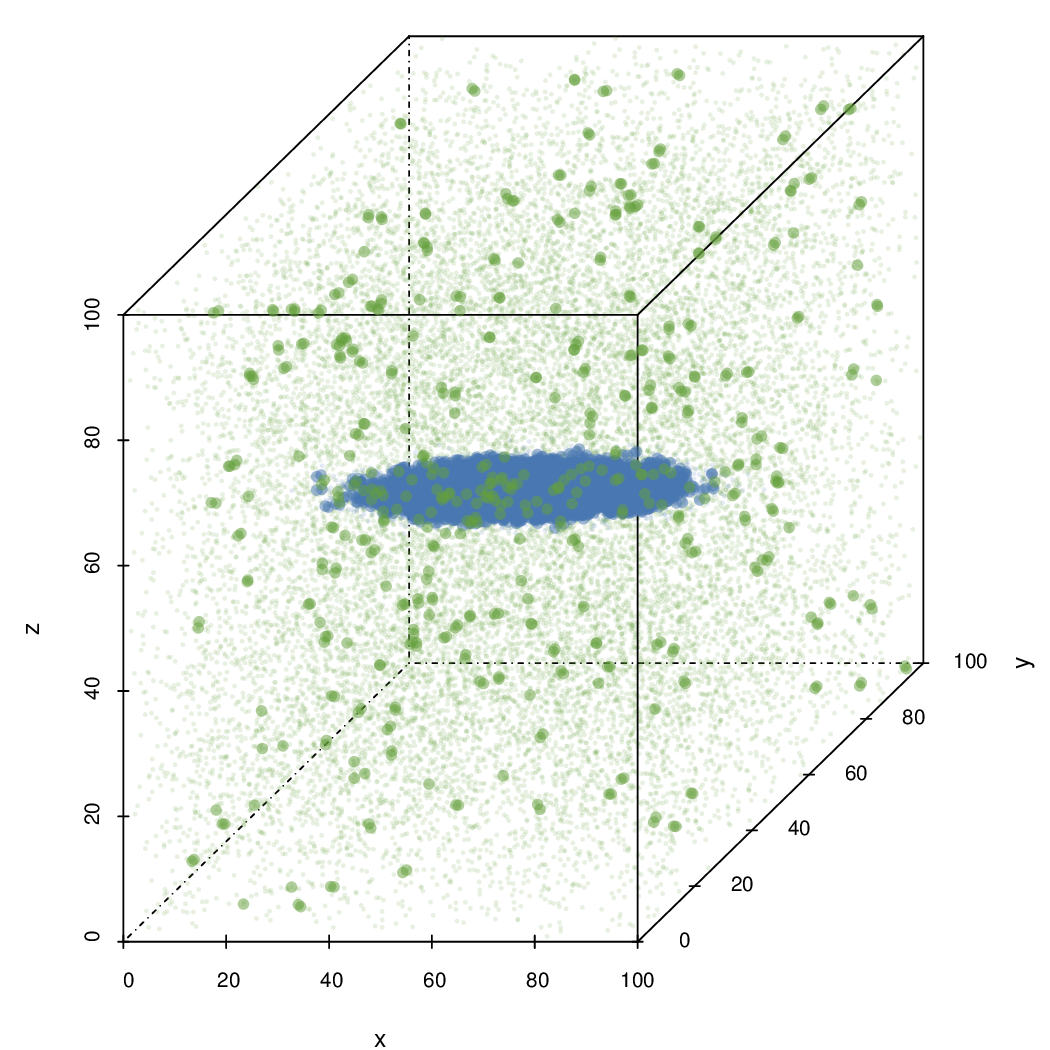
\includegraphics[keepaspectratio=true, width=\textwidth, height=0.23\textheight]{discussion/img/baakman_5_abs_error_mbeSmallerThansambe}
				\caption{Data set \baakmanFive}
				\label{fig:discussion:performance:mbeLowerError:baakman5}
			\end{subfigure}			
			\caption{Low opacity scatter plot of set %
				\subref{fig:discussion:performance:mbeLowerError:ferdosi1} \ferdosiOne, %
				\subref{fig:discussion:performance:mbeLowerError:baakman1} \baakmanOne, %
				\subref{fig:discussion:performance:mbeLowerError:baakman4} \baakmanFour, and %
				\subref{fig:discussion:performance:mbeLowerError:baakman5} \baakmanFive, %
				with an overlay of larger, colored points where the absolute error of \sambe is greater than or equal to that of \mbe.}
			\label{fig:discussion:performance:singleSphere:mbeLowerError}
		\end{figure}
		%	
		The plots in \cref{fig:discussion:performance:singleSphere:mbeLowerError} emphasize the points in data set \ferdosiOne and \baakmanOne where the absolute error of \mbe is smaller than that of \sambe. These plots show that the shape-adaptive kernels outperform symmetric kernels near the borders of the data sets.
			% Why the boundary effect
			We expect that this boundary effect is due to the strong anisotropy of the local neighborhood of the points near the limits of the data sets. Consequently the domain of the shape-adaptive kernels extends less outside of the boundaries of the data set than the domains of the symmetric kernels. This results in less underestimation of densities near the boundary of the data set, if shape-adaptive kernels are used.
			% Why is it stonger of the Gaussian is more anisotropic
			Furthermore the strength of the boundary effect seems to increase as the Gaussian component of the data set is more anisotropic. However the seemingly better performance of \sambe is due to an increase in the number of points where the density estimated by \sambe equals the density estimated by \mbe. In data set \ferdosiOne the two estimators give a different result on all points. In data set \baakmanOne the estimators agree on the density of \percentage{1.327294605254362e+01} of the points, this increases to \percentage{3.535329901731399e+01} in data set \baakmanFive.
			%SAMBE == MBE
			%Ferdosi 1 (0.000000000000000e+00 percent)
			%Baakman 1 (1.327294605254362e+01 percent)
			%Baakman 4 (2.989838892974129e+01 percent)
			%Baakman 5 (3.535329901731399e+01 percent)
			As the Gaussian component becomes more anisotropic the number of points whose local neighborhood consists only of uniform noise increases. On average the covariance matrix of neighborhoods that contain primarily points sampled from the noise component should be scalar. Consequently as the anisotropy of the Gaussian component increases more shape-adaptive kernels take on a shape that is near-symmetric. This results in points were both estimators give the same approximated density. 
	
	% Multi Sphere
		\begin{figure}
			\centering
			\begin{subfigure}{0.23\textwidth}
				\centering
				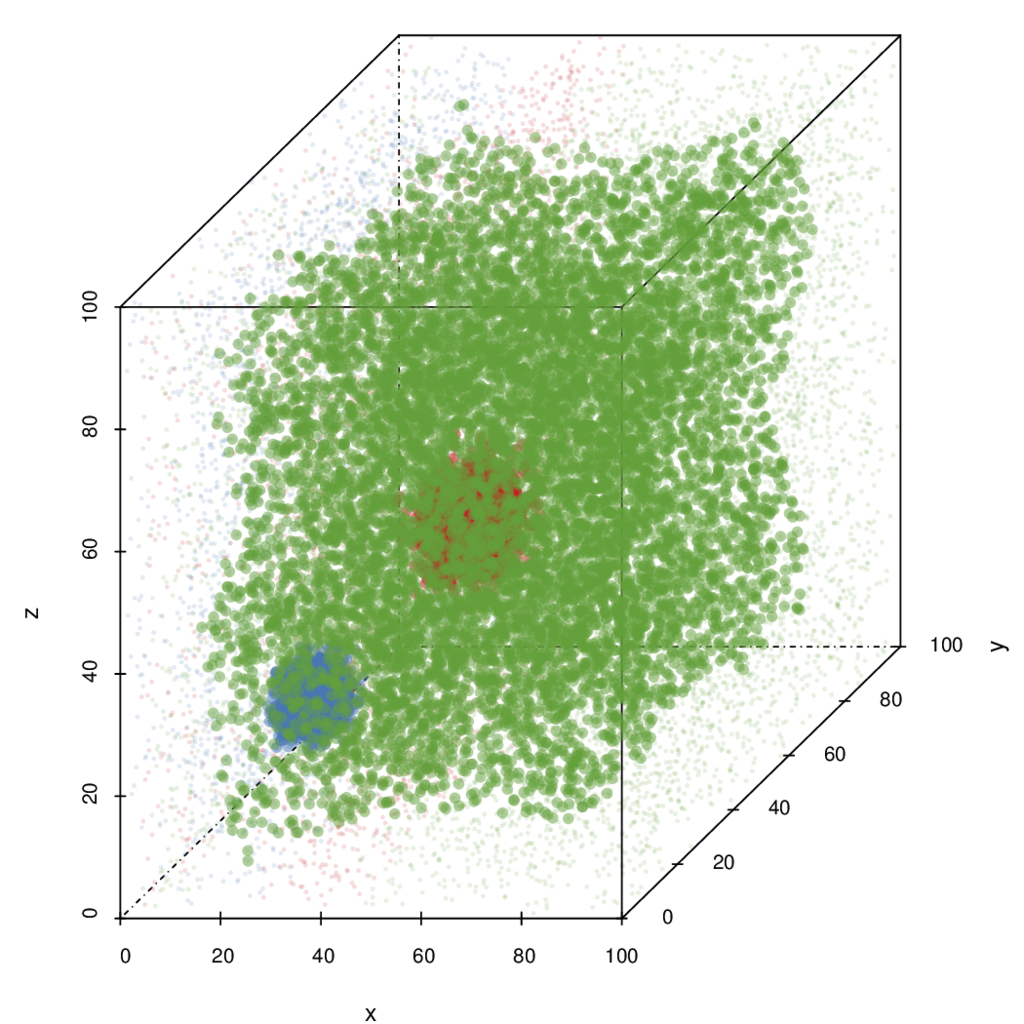
\includegraphics[keepaspectratio=true, width=\textwidth, height=0.23\textheight]{discussion/img/ferdosi_2_abs_error_mbeSmallerThansambe}
				\caption{Data set \ferdosiTwo}
				\label{fig:discussion:performance:mbeLowerError:ferdosi2}
			\end{subfigure}
			\begin{subfigure}{0.23\textwidth}
				\centering
				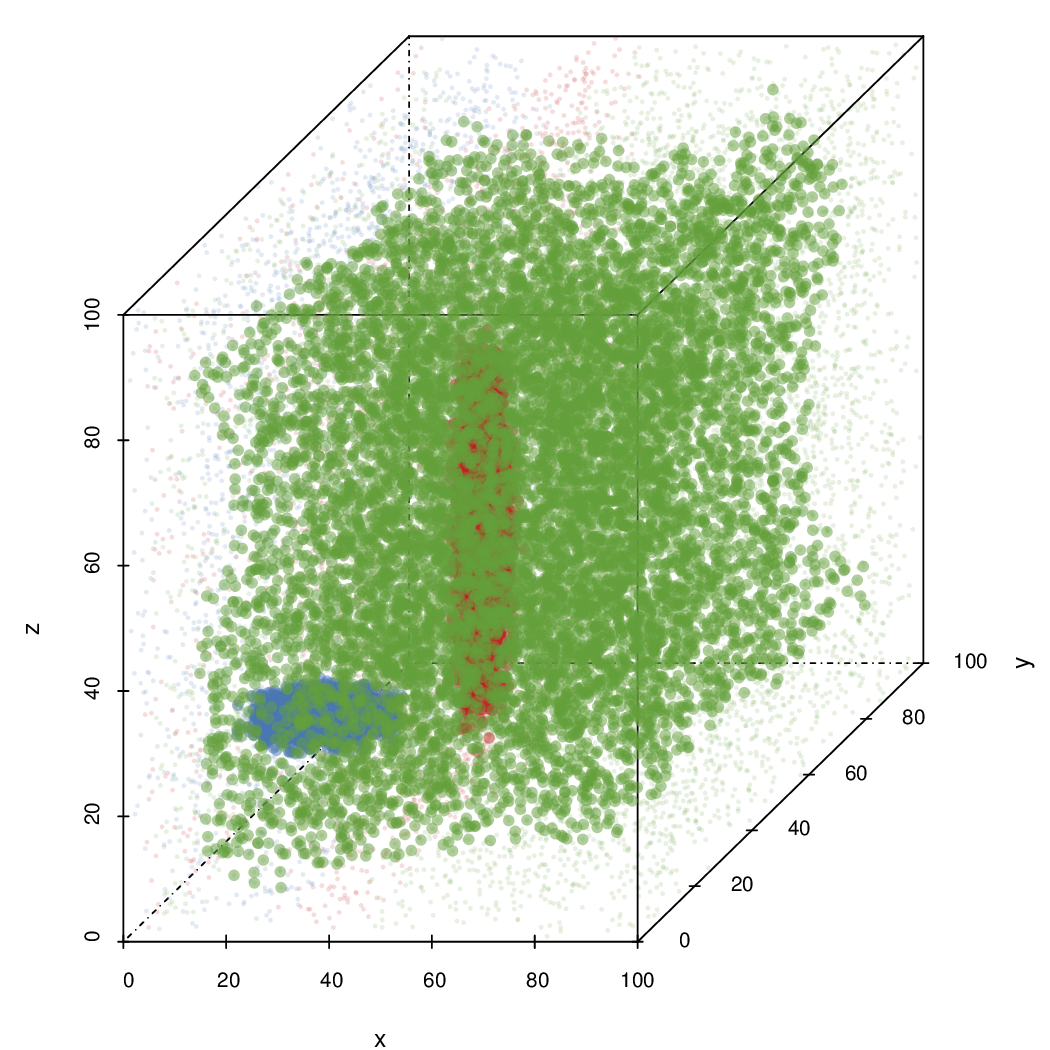
\includegraphics[keepaspectratio=true, width=\textwidth, height=0.23\textheight]{discussion/img/baakman_2_abs_error_mbeSmallerThansambe}
				\caption{Data set \baakmanTwo}
				\label{fig:discussion:performance:mbeLowerError:baakman2}
			\end{subfigure}	
			\subfigvspace
			\begin{subfigure}{0.23\textwidth}
				\centering
				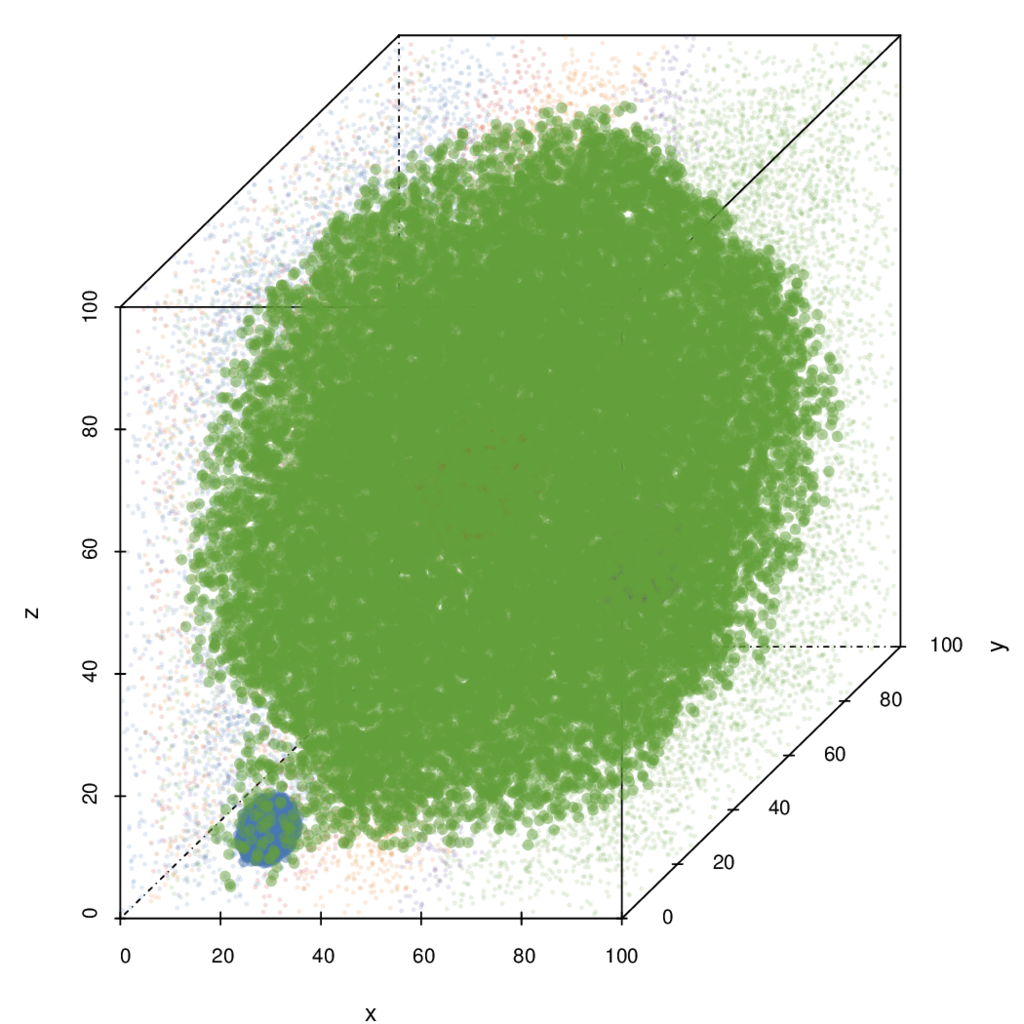
\includegraphics[keepaspectratio=true, width=\textwidth, height=0.23\textheight]{discussion/img/ferdosi_3_abs_error_mbeSmallerThansambe}
				\caption{Data set \ferdosiThree}
				\label{fig:discussion:performance:mbeLowerError:ferdosi3}
			\end{subfigure}
			\begin{subfigure}{0.23\textwidth}
				\centering
				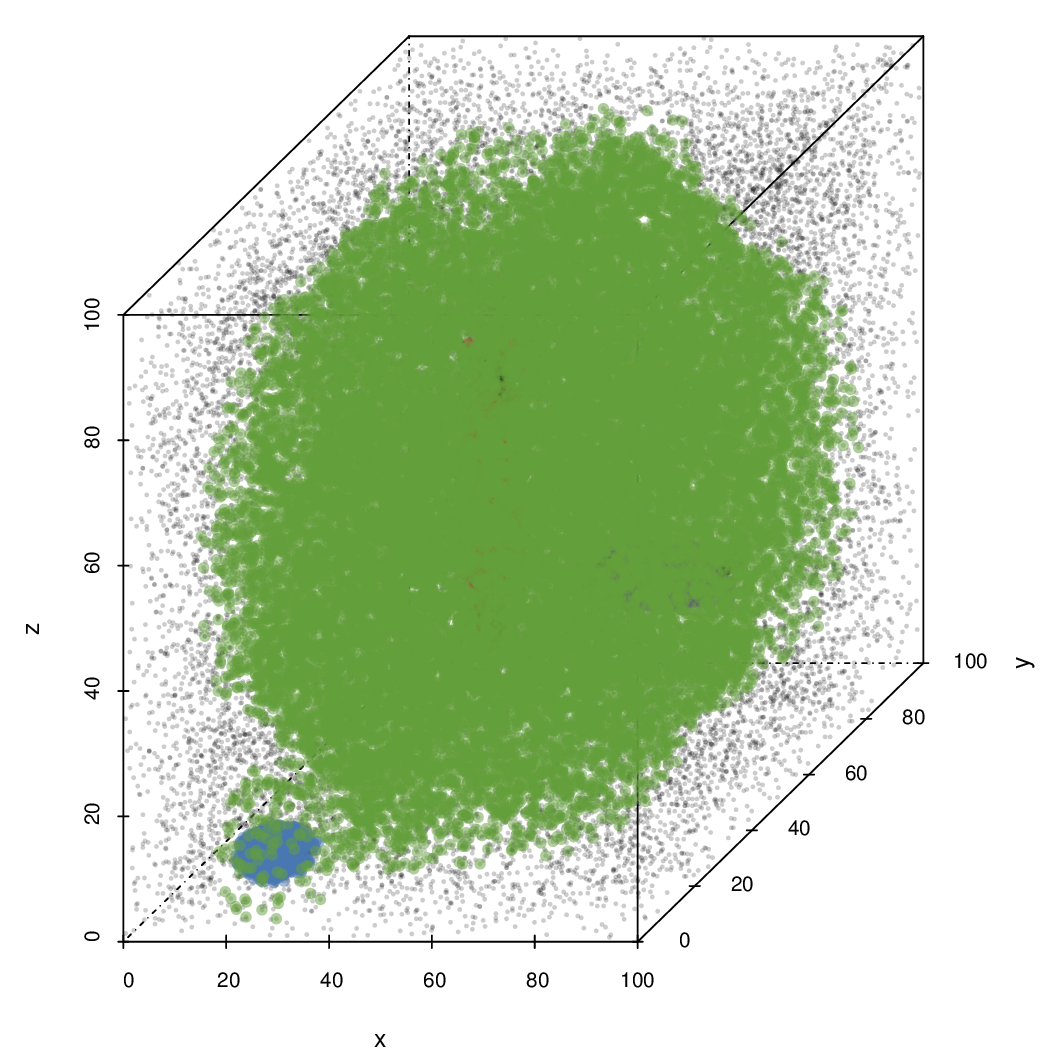
\includegraphics[keepaspectratio=true, width=\textwidth, height=0.23\textheight]{discussion/img/baakman_3_abs_error_mbeSmallerThansambe}
				\caption{Data set \baakmanThree}
				\label{fig:discussion:performance:mbeLowerError:baakman3}
			\end{subfigure}			
			\caption{Low opacity scatter plot of data set %
				\subref{fig:discussion:performance:mbeLowerError:ferdosi2} \ferdosiTwo, %
				\subref{fig:discussion:performance:mbeLowerError:baakman2} \baakmanTwo, %
				\subref{fig:discussion:performance:mbeLowerError:ferdosi3} \ferdosiThree, and %
				\subref{fig:discussion:performance:mbeLowerError:baakman3} \baakmanThree %
				with an overlay of high opacity, larger points where the absolute error of \mbe is smaller than that of \sambe.}
			\label{fig:discussion:performance:multisphere:mbeLowerError}
		\end{figure}	
		The points where using fixed-shape kernels results in a smaller error in data sets \ferdosiTwo through \baakmanThree are emphasized in
		\cref{fig:discussion:performance:multisphere:mbeLowerError}. We contribute the boundary effect in these data sets to the same cause as the boundary effect in the data sets with a single Gaussian component. Interestingly the points in data set \ferdosiThree and \baakmanThree where the absolute error of \mbe is lower, approximate a sphere, contrary to the cube they define for data set \ferdosiTwo and \baakmanTwo. It is our expectation that this is caused by the smaller distance between the means of the Gaussian components and the range of the uniform random background in \ferdosiThree and \baakmanThree.
			% Define Ferdosi 3 Noise
			To test this we define data set \ferdosiThreeNoise, which replaces the uniform random background of \ferdosiThree with $\uniformDist{[-20, -20, -20]}{[120, 120, 120]}$. We adjust the number of points sampled from this component to ensure that its density is equal to that of the noise component of \ferdosiThree.
			% Is there any effect on the MSE
			The overall \mse of both estimators is slightly smaller for data set \ferdosiThreeNoise than for \ferdosiThree, however the \mse of `Trivariate Gaussian 1' and 3 shows a small increase. 
			% Did the distance to the boundaries explain it?
			\Cref{fig:discussion:ferdosi3Noise:mbeLowerError} confirms that the spherical shape in \cref{fig:discussion:performance:mbeLowerError:ferdosi3,fig:discussion:performance:mbeLowerError:baakman3} is caused by the Gaussian near the boundary of the data set. As the shape defined by the emphasized points is now a cubical instead of spherical. 
			% The Plots of Ferdosi 3 Noise
			\begin{figure}[b!]
				\centering
				\begin{subfigure}{0.23\textwidth}
					\centering
					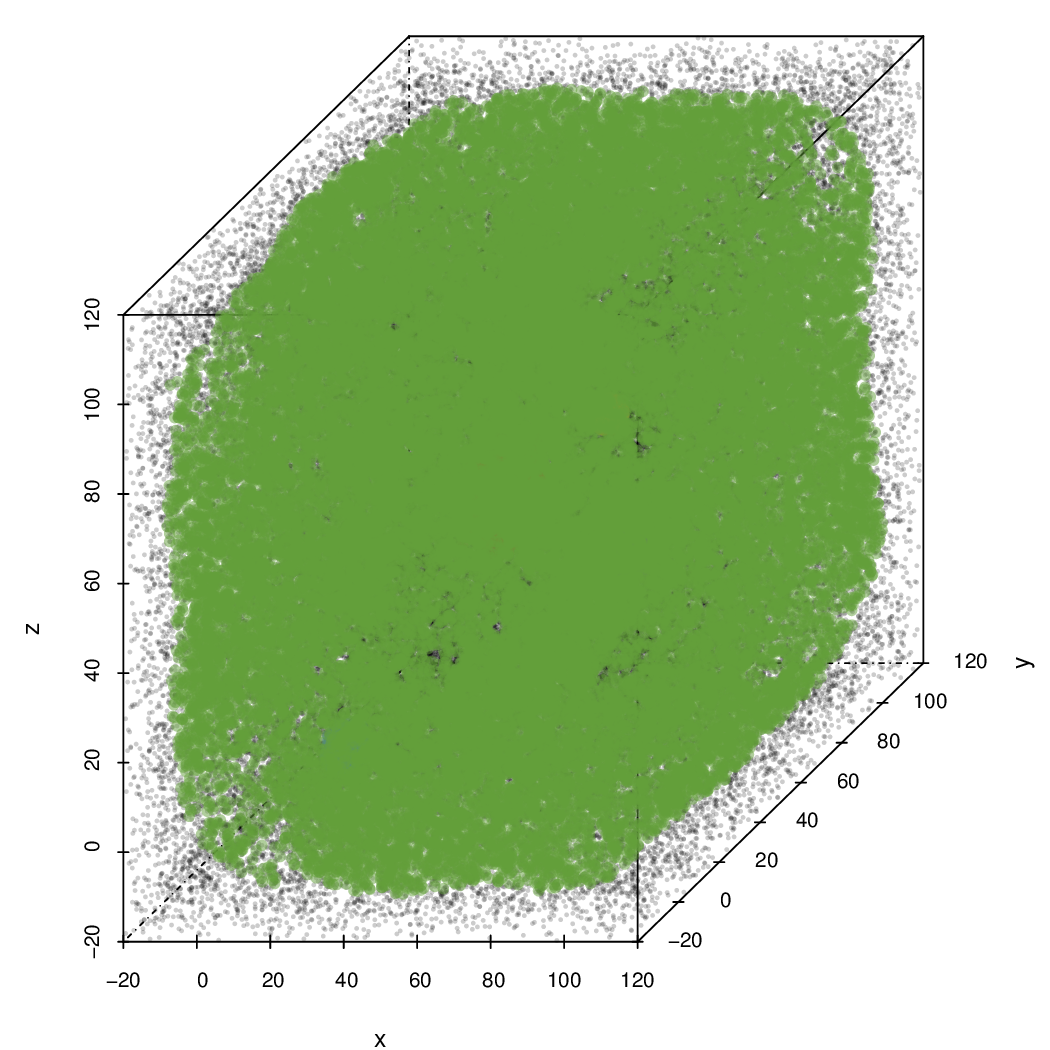
\includegraphics[keepaspectratio=true, width=\textwidth, height=0.23\textheight]{discussion/img/ferdosi_3_more_noise_abs_error_mbeSmallerThansambe.png}
					\caption{Absolute Error}
					\label{fig:discussion:ferdosi3Noise:mbeLowerError}
				\end{subfigure}		
				\begin{subfigure}{0.23\textwidth}
					\centering
					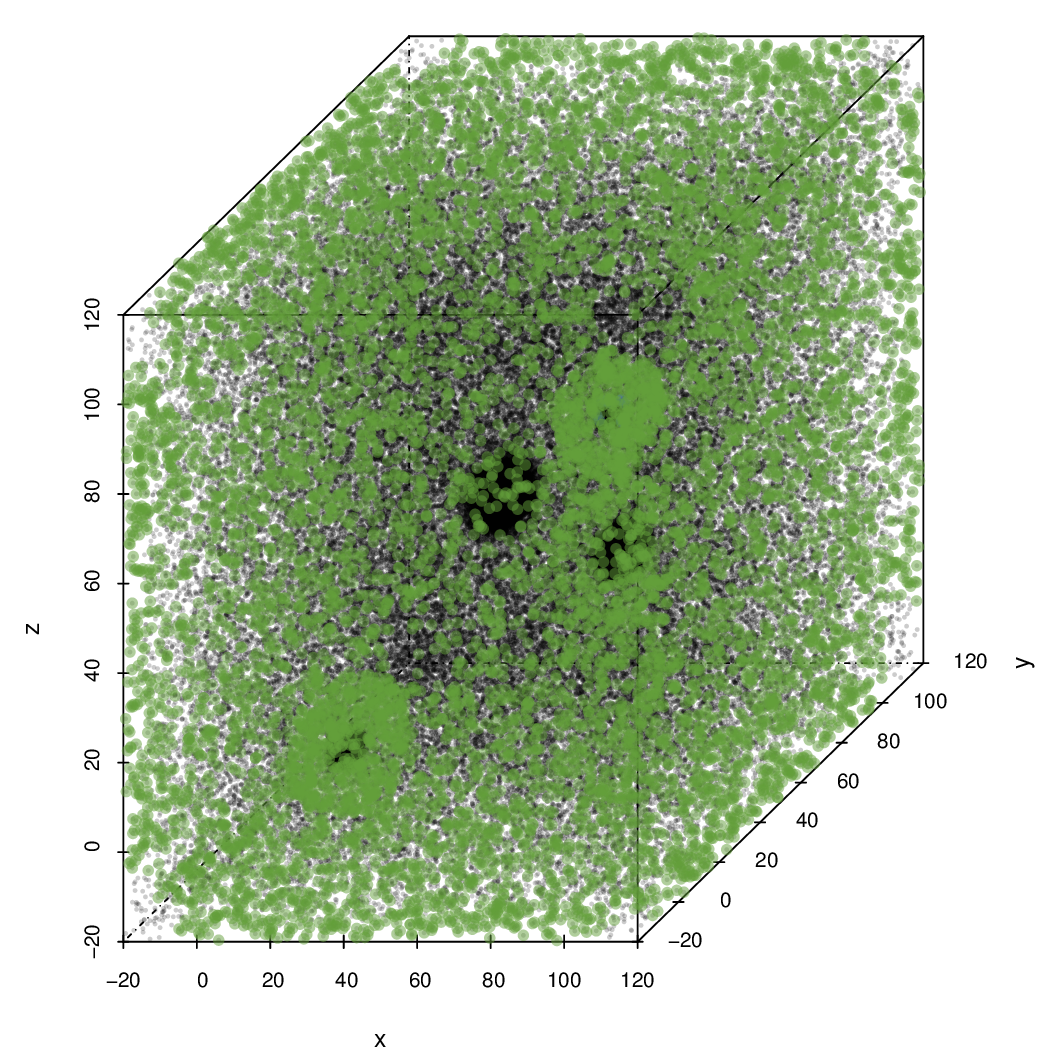
\includegraphics[keepaspectratio=true, width=\textwidth, height=0.23\textheight]{discussion/img/ferdosi_3_more_noise_anisotropy.png}
					\caption{Anisotropy}
					\label{fig:discussion:ferdosi3Noise:anisotropy}
				\end{subfigure}			
				\caption{Low opacity scatter plot of data set \ferdosiThreeNoise with %
					\subref{fig:discussion:ferdosi3Noise:mbeLowerError} points where the absolute error of \mbe is lower than that of \sambe and %
					\subref{fig:discussion:ferdosi3Noise:anisotropy} points sampled from the Gaussian components with kernels whose anisotropy falls in the \nth{95} percentile of the complete data set emphasized.}
				\label{fig:discussion:ferdosi3Noise}
			\end{figure}		

% Some conclusion
To conclude we have found that shape-adaptive kernels definitely improve performance in some cases, \ie near the boundary of the data sets and near the mean of some Gaussian components. Unfortunately in other cases the anisotropic kernels are detrimental. The difference in \mse between the two estimators shows that generally, using fixed-shape kernels is slightly advantageous. 

\subsection{Kernel Anisotropy}
\label{s:discussion:anisotropy}
%!TEX root = ../paper.tex

% Small differences in anisotropy  
	In \cref{s:results} some small differences between the anisotropies of the different kernels were observed. In this section we attempt to find an explanation for the lack of dissimilarity between the estimators.

	% Single Sphere
			\begin{figure}
				\centering
				\begin{subfigure}{0.23\textwidth}
					\centering
					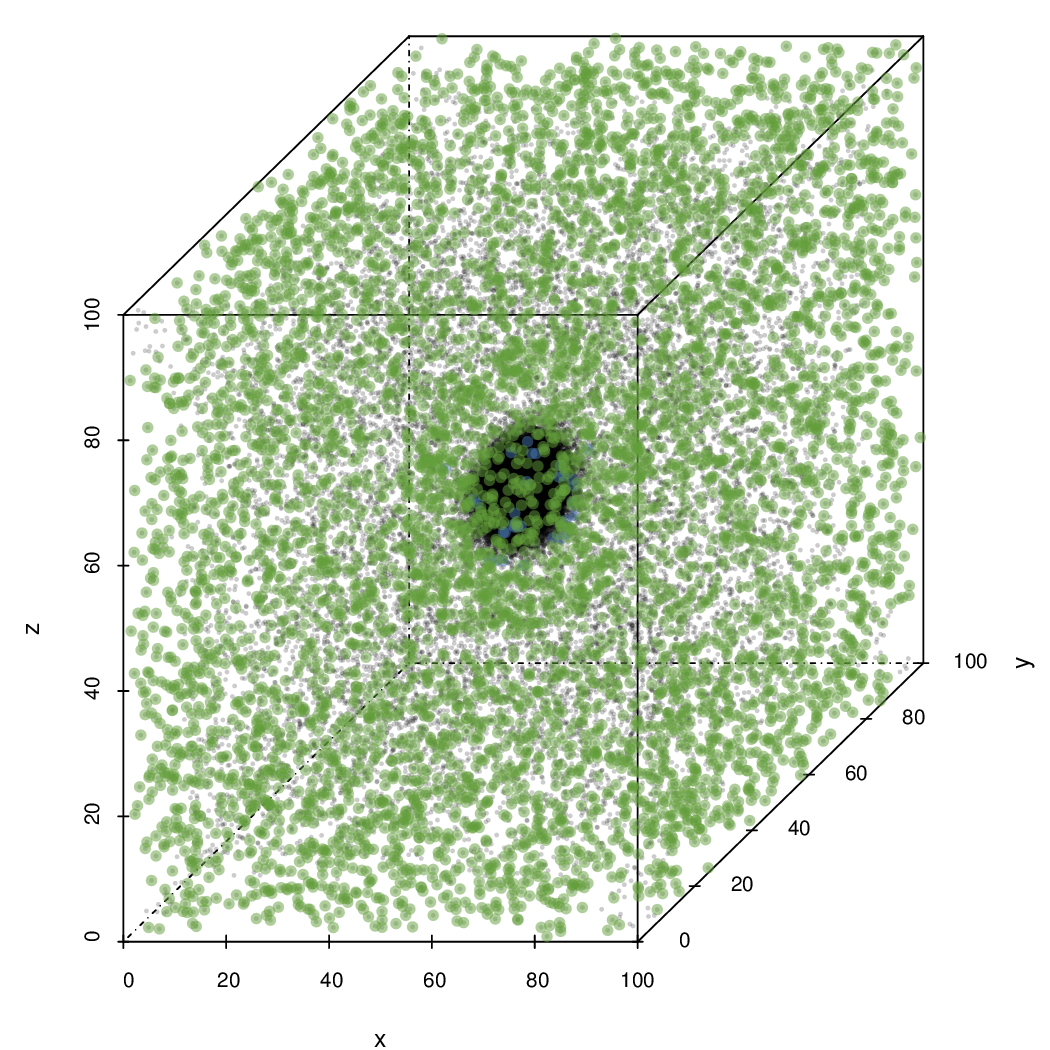
\includegraphics[keepaspectratio=true, width=\textwidth, height=0.23\textheight]{discussion/img/ferdosi_1_60000_anisotropy.png}
					\caption{\ferdosiOne [\num{2.783732800937043e+00}, \num{4.876641609906343e+00}]}
					\label{fig:discussion:anisotropy:ferdosi1}
				\end{subfigure}
				\begin{subfigure}{0.23\textwidth}
					\centering
					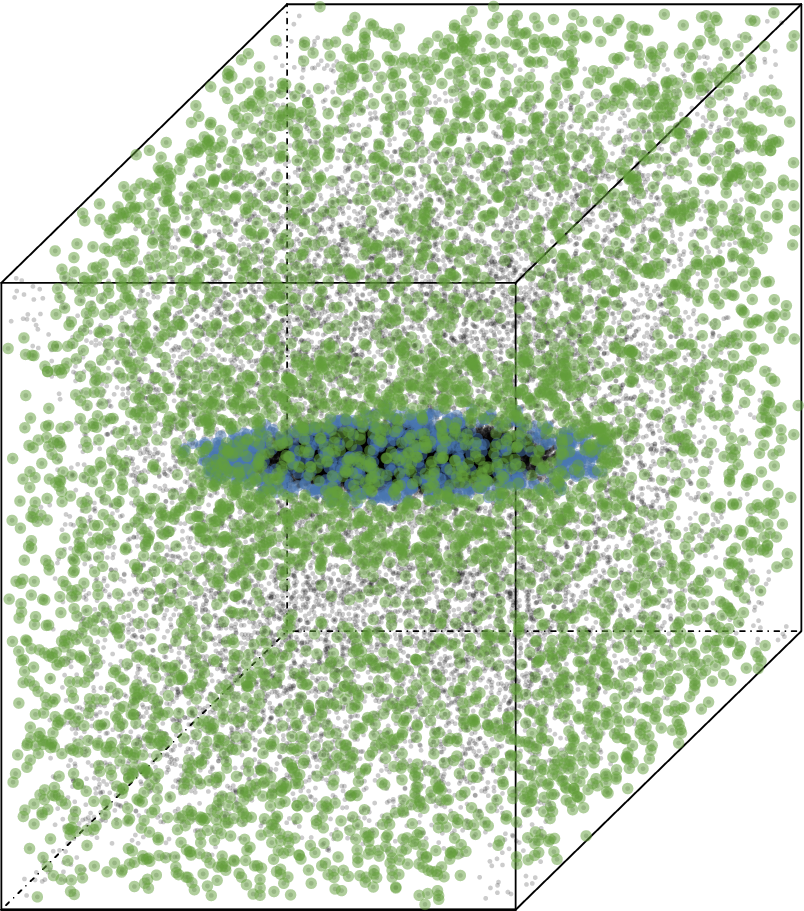
\includegraphics[keepaspectratio=true, width=\textwidth, height=0.23\textheight]{discussion/img/baakman_1_60000_anisotropy.png}
					\caption{\baakmanOne [\num{2.955638611296131e+00}, \num{4.876641609906340e+00}]}
					\label{fig:discussion:anisotropy:baakman1}
				\end{subfigure}	
				\subfigvspace
				\begin{subfigure}{0.23\textwidth}
					\centering
					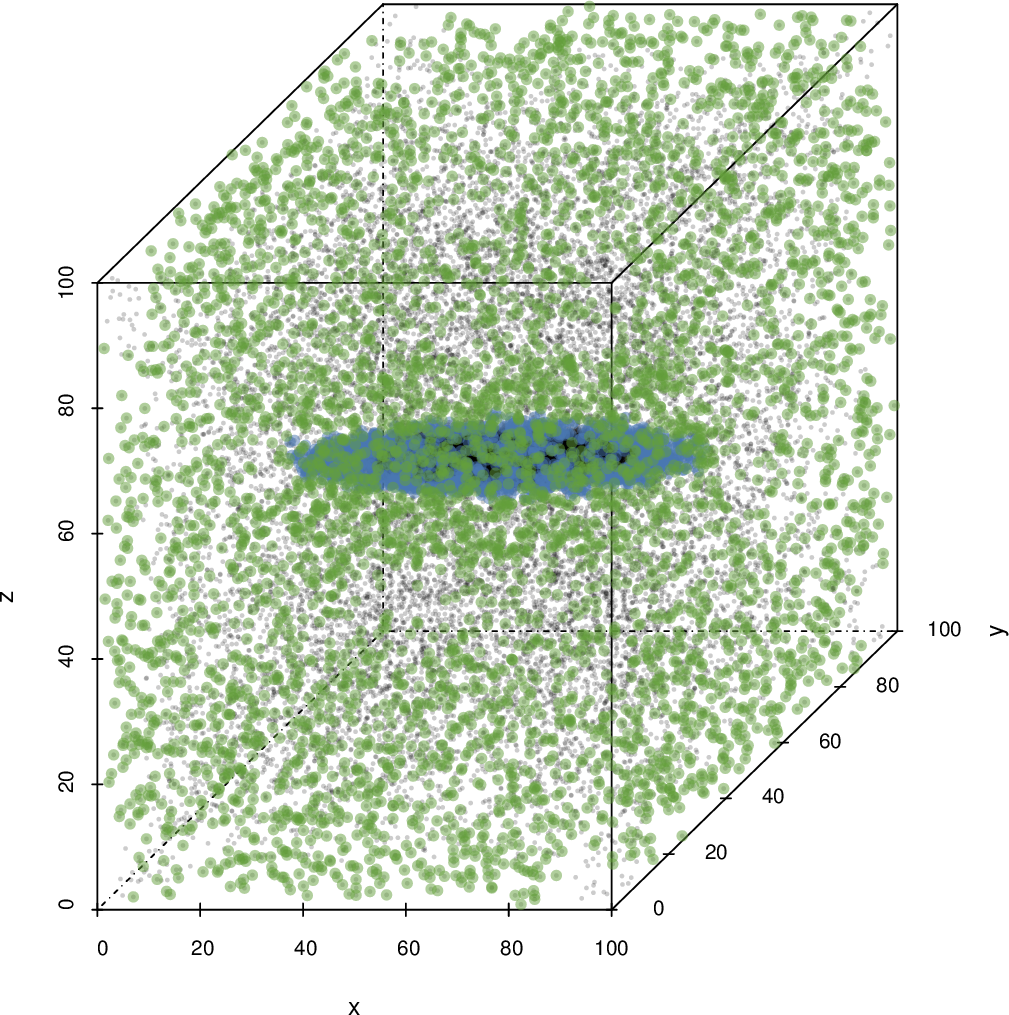
\includegraphics[keepaspectratio=true, width=\textwidth, height=0.23\textheight]{discussion/img/baakman_4_60000_anisotropy.png}
					\caption{\baakmanFour [\num{3.105833113039985e+00}, \num{5.987200775539245e+00}]}
					\label{fig:discussion:anisotropy:baakman4}
				\end{subfigure}		
				\begin{subfigure}{0.23\textwidth}
					\centering
					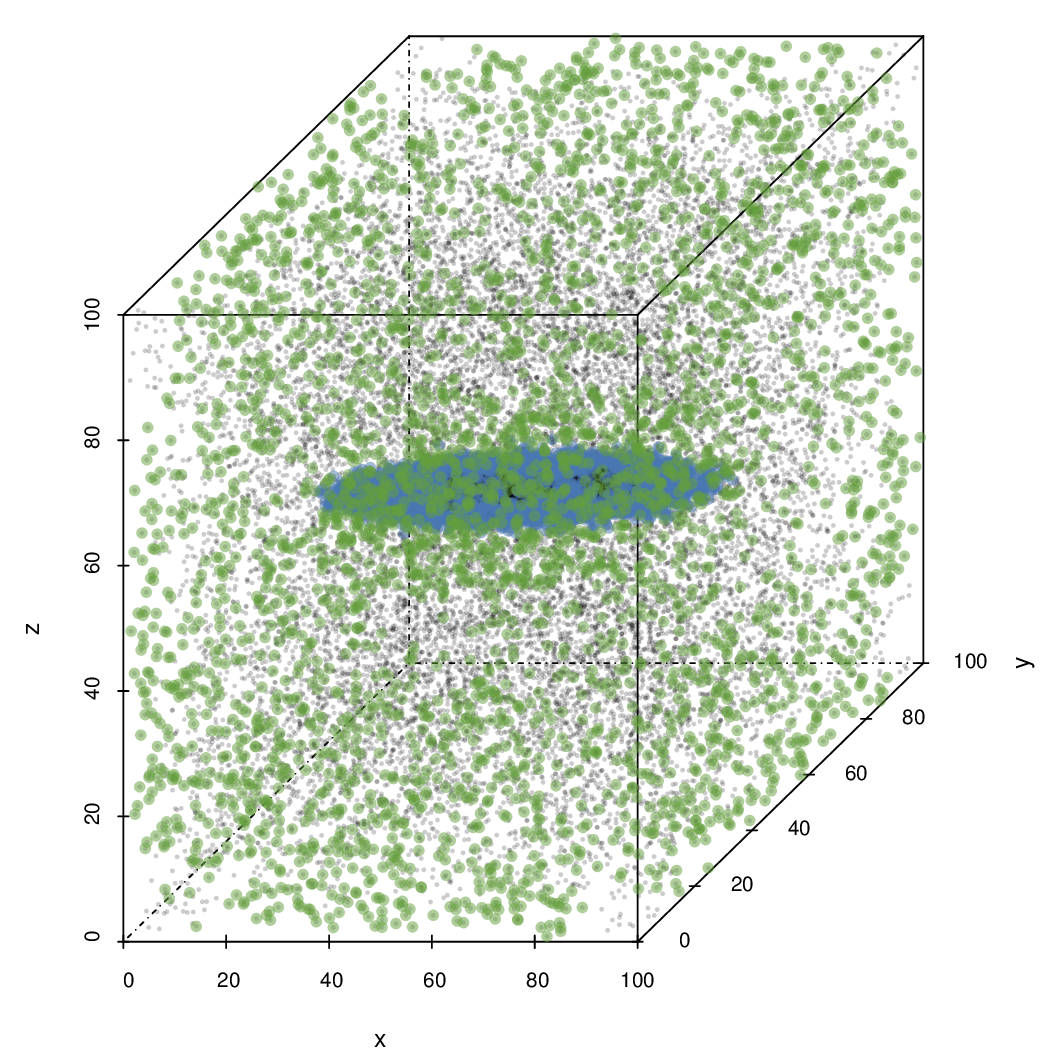
\includegraphics[keepaspectratio=true, width=\textwidth, height=0.23\textheight]{discussion/img/baakman_5_60000_anisotropy.png}
					\caption{\baakmanFive [\num{3.546238846198991e+00}, \num{8.192210308245695e+00}]}
					\label{fig:discussion:anisotropy:baakman5}
				\end{subfigure}			
				\caption{Scatter plots of data set
					\subref{fig:discussion:anisotropy:ferdosi1} \ferdosiOne, %
					\subref{fig:discussion:anisotropy:baakman1} \baakmanOne, %
					\subref{fig:discussion:anisotropy:baakman4} \baakmanFour, and %
					\subref{fig:discussion:anisotropy:baakman5} \baakmanFive. %
					The points with kernels whose anisotropy lies in the \nth{90} percentile are shown larger, and colored. The anisotropy range of the kernels of the emphasized points is shown below the plots.}
				\label{fig:discussion:anisotropy:singleSphere}
			\end{figure}
			%	
			\Cref{fig:discussion:anisotropy:singleSphere} shows the data sets with a single Gaussian with points whose anisotropy lie in the \nth{90} percentile emphasized. 
				% Ferdosi 1 & Baakman 1
				Hardly any differences are visible between the plots of data set \ferdosiOne and \baakmanOne. 
					% Very few points from Gaussian comonent
					In \cref{fig:discussion:anisotropy:ferdosi1,fig:discussion:anisotropy:baakman1} \percentage{5.180481283422460e-01} and \percentage{1.174799465240642e+01}, respectively, of the emphasized points are sampled from the Gaussian component of the data sets. This shows that the kernels in data set \baakmanOne are influenced by the increase in anisotropy compared to the isotropy of the Gaussian component in data set \ferdosiOne.
					% Shell of points sampled from the noise around the Gaussian comonent
					Furthermore a shell of points sampled from the noise with kernels whose anisotropy is relatively high surrounds the Gaussian component. It is quite likely that the shape of these kernels is influenced by the Gaussian component.
					% Explanation: high density -> anisotropy detection fails
					We expect that nearer to the mean of the Gaussian component fewer kernels are influenced by its anisotropy as the physical density of points is quite high in that area. Consequently the volume of the local neighborhood is quite low and thus possibly insufficient to represent the shape of the Gaussian.
				% Baakman 4 and 5
				In data set \baakmanFour and \baakmanFive a larger percentage of the points with a kernel whose anisotropy is relatively high is sampled from the Gaussian component, \percentage{2.190842245989305e+01} and \percentage{4.207887700534759e+01}, respectively. 
				% Conclusion
				Therefore we tentatively conclude that as the anisotropy of the Gaussian component increases, the anisotropy of the kernels of the points near that component increases as well.
		
	% Multi Sphere
		\begin{figure}
			\centering
			\begin{subfigure}{0.23\textwidth}
				\centering
				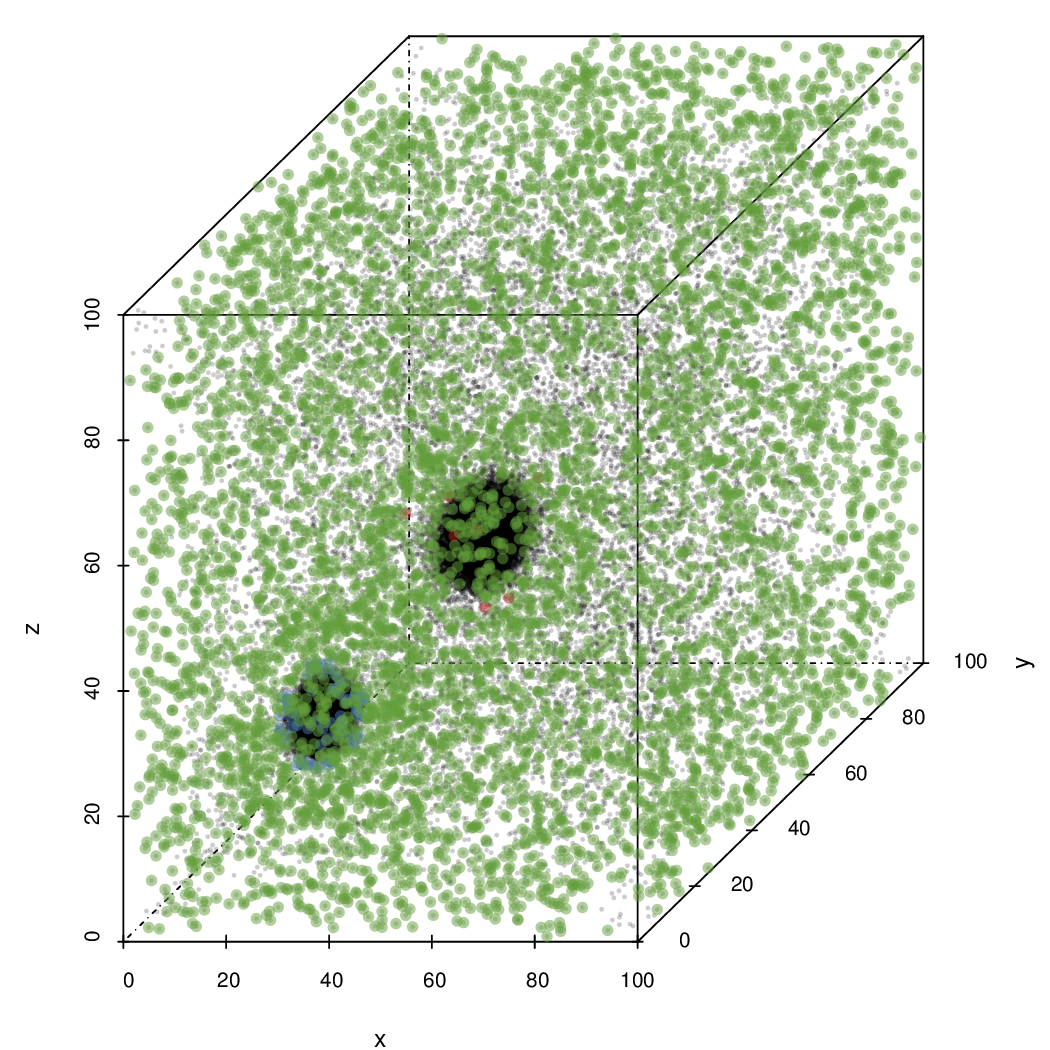
\includegraphics[keepaspectratio=true, width=\textwidth, height=0.23\textheight]{discussion/img/ferdosi_2_60000_anisotropy.png}
				\caption{\ferdosiTwo [\num{2.215970619635167e+00}, \num{5.678002691654005e+00}]}
				\label{fig:discussion:anisotropy:ferdosi2}
			\end{subfigure}
			\begin{subfigure}{0.23\textwidth}
				\centering
				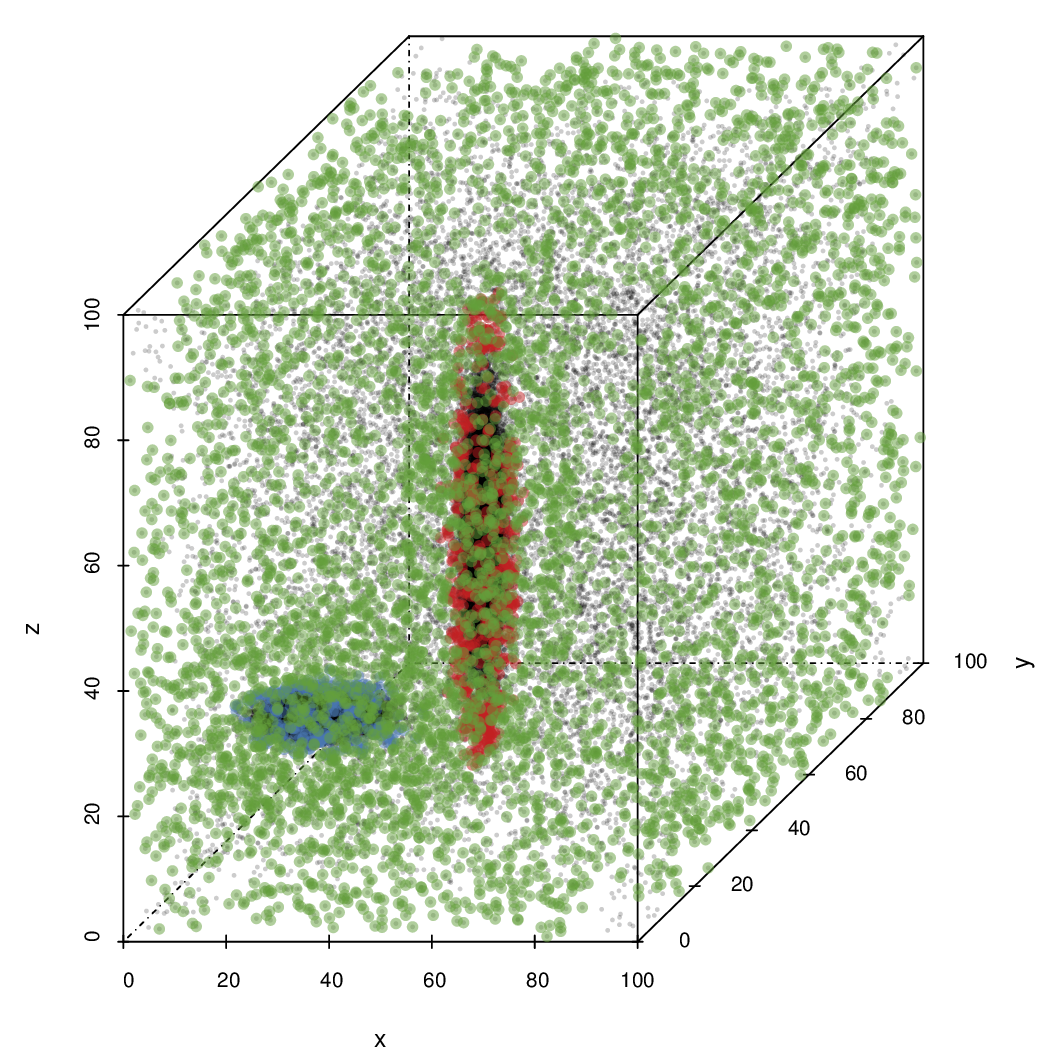
\includegraphics[keepaspectratio=true, width=\textwidth, height=0.23\textheight]{discussion/img/baakman_2_60000_anisotropy.png}
				\caption{\baakmanTwo [\num{2.463414286522871e+00}, \num{7.134567710248723e+00}]}
				\label{fig:discussion:anisotropy:baakman2}
			\end{subfigure}	
			\subfigvspace
			\begin{subfigure}{0.23\textwidth}
				\centering
				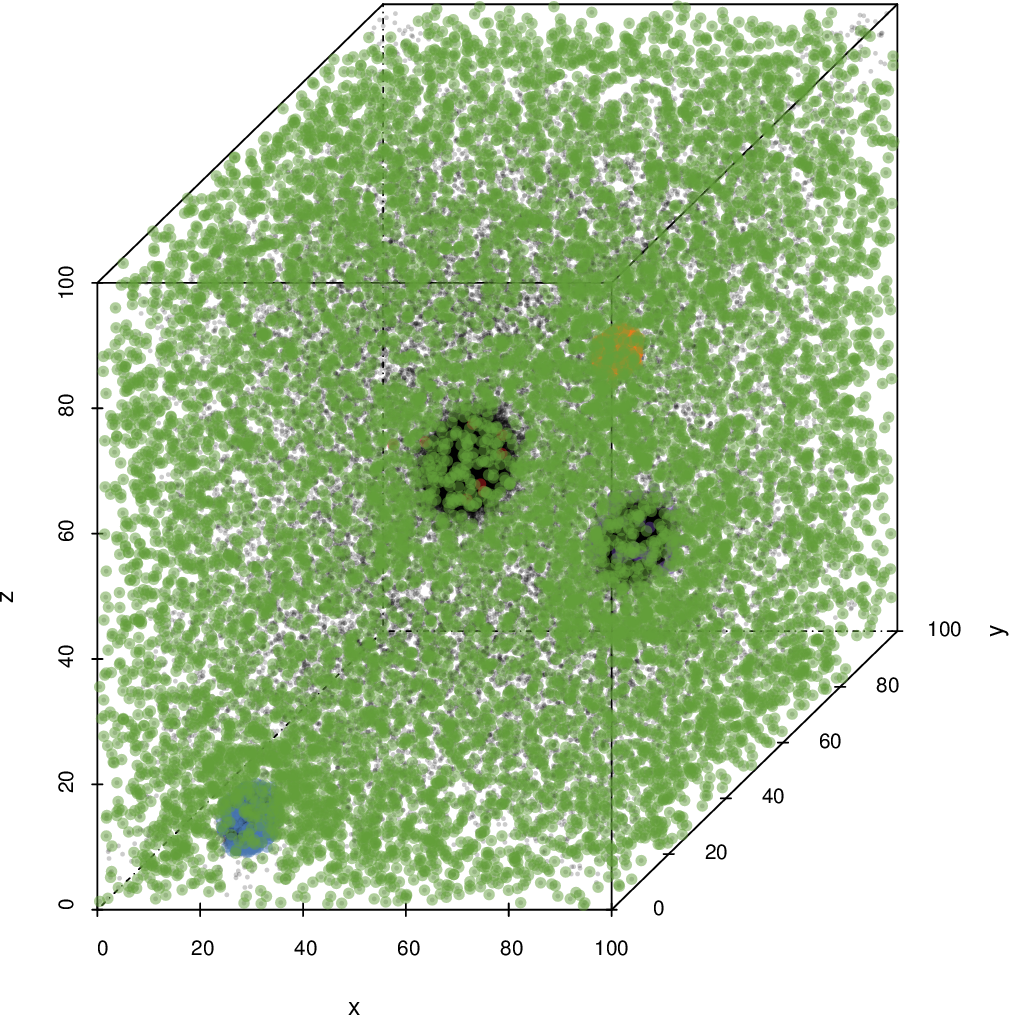
\includegraphics[keepaspectratio=true, width=\textwidth, height=0.23\textheight]{discussion/img/ferdosi_3_120000_anisotropy.png}
				\caption{\ferdosiThree [\num{2.138909227329211e+00}, \num{8.855946762727447e+00}]}
				\label{fig:discussion:anisotropy:ferdosi3}
			\end{subfigure}		
			\begin{subfigure}{0.23\textwidth}
				\centering
				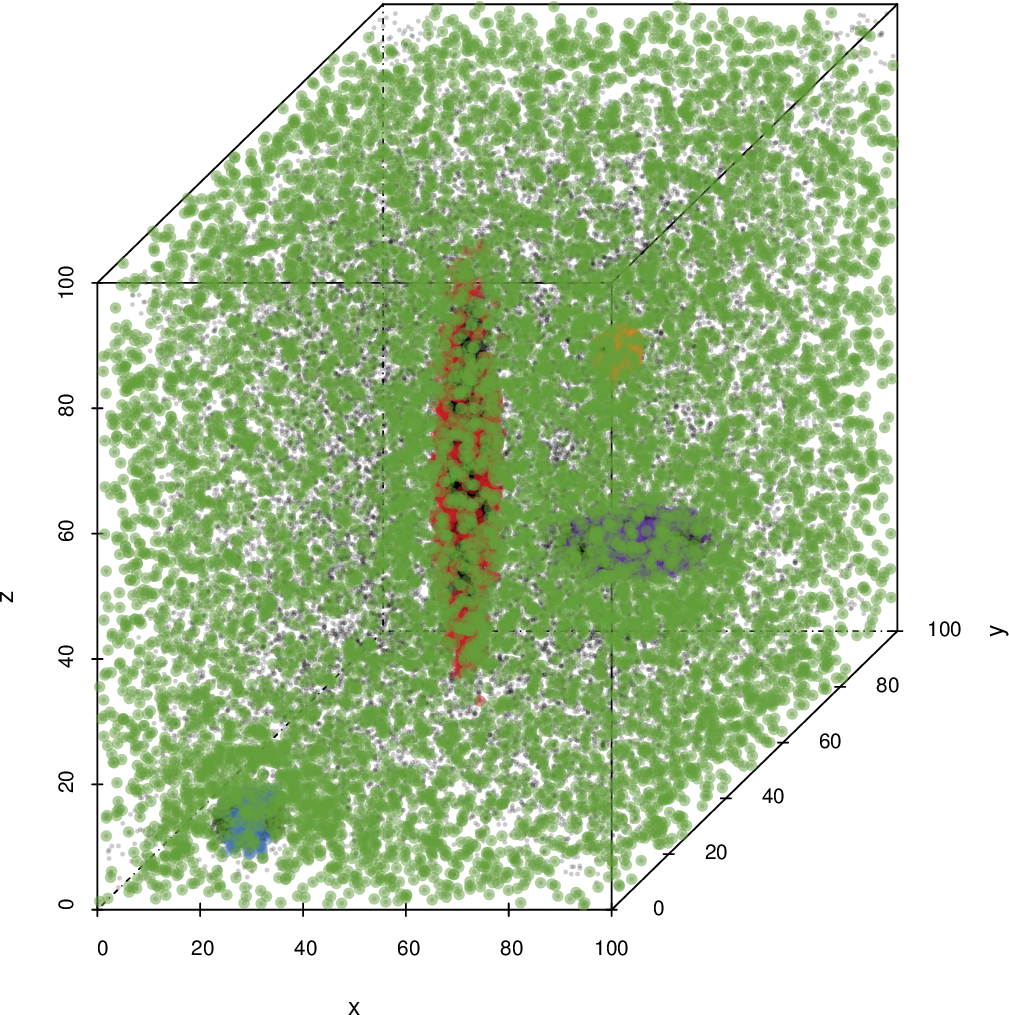
\includegraphics[keepaspectratio=true, width=\textwidth, height=0.23\textheight]{discussion/img/baakman_3_60000_anisotropy.png}
				\caption{\baakmanThree [\num{2.316497642958064e+00}, \num{8.855946762727445e+00}]}
				\label{fig:discussion:anisotropy:baakman3}
			\end{subfigure}			
			\caption{Scatter plots of set
				\subref{fig:discussion:anisotropy:ferdosi2} \ferdosiTwo, %
				\subref{fig:discussion:anisotropy:baakman2} \baakmanTwo, %
				\subref{fig:discussion:anisotropy:ferdosi3} \ferdosiThree, and %
				\subref{fig:discussion:anisotropy:baakman3} \baakmanThree. %
				The points that have an anisotropy in the \nth{90} percentile are shown larger and colored. Below each plot the range of the anisotropy of the kernels of the emphasized points is shown.}
			\label{fig:discussion:anisotropy:multisphere}
		\end{figure}			
		% General Introduction
		\Cref{fig:discussion:anisotropy:multisphere} emphasizes the points with the most anisotropic kernels in data set \ferdosiTwo through \baakmanThree. 
		% Ferdosi 2
			% Same observations as for ferdosi 1, present percentages
			In the plot associated with data set \ferdosiTwo we observe the same shells of points with highly anisotropic kernels around the Gaussian components as in data set \ferdosiOne. Another similarity between these two data sets is that very few points sampled from the Gaussian component have a kernel with high anisotropy; \percentage{1.453877} and \percentage{0.1169786} of the points with a high anisotropy are sampled from the first and second Gaussian component, respectively. 
			% F2G1 vs F2G2
			We contribute the difference in the number of highly anisotropic kernels associated with data points sampled from the two Gaussian components to the difference in the volume of the their eigenspheres.
		% Baakman 2
			% More points near the Gaussian anisotropic
			For \cref{fig:discussion:anisotropy:baakman2} we find that the increase in anisotropy of the components causes \percentage{4.328209} and \percentage{8.656417} of the kernels with high anisotropy to be associated with a point sampled from `Trivariate Gaussian 1' and 2, respectively. 
		% Ferdosi 3
			% G1 and G3 have anisotropic kernels. 
			Interestingly in data set \ferdosiThree, two of the four spherical Gaussians, `Trivariate Gaussian 1' and 3, are associated with respectively \percentage{1.404095} and \percentage{2.223151} of the highly anisotropic kernels. Whereas no point sampled from `Trivariate Gaussian 2' or 4 has a kernel with high anisotropy.
			% Relate to results: components with highest sd, lowest means, lower density -> larger variation in anisotropy
			Comparing the mean kernel anisotropy in \cref{tab:results:multiSphere:anisotropy} we find that relative to the other Gaussian components in \ferdosiThree, `Trivariate Gaussian 1' and 3 have a relatively low mean anisotropy. However their standard deviations are relatively high, suggesting that in these components some kernels are extremely anisotropic, whereas others are near isotropic. We contribute this difference within the points sampled from these Gaussian components to differences in the physical densities of the neighborhoods around the means, as we did for data set \ferdosiOne and \baakmanOne.
			% Why G1 and G3 and not G2 and G4? 
			Component one and four of data set \ferdosiThree differ from the other Gaussian components in two aspects: firstly the volume of their eigenspheres is relatively low and secondly they are placed near the boundaries of the data set. 
				% G1/G3 are placed near the  border of the data set, contrast with results of F3Noise?
				\Cref{fig:discussion:ferdosi3Noise:anisotropy} shows that the distance to the limits of the background does not explain the difference in anisotropy of the kernel, as in that figure the first and third component of \ferdosiThreeNoise have more anisotropic kernels than the other components, even though they are farther away from the boundary of the data set.
				% G1/G3 have lower covariance:
				The first explanation fits with the observations from \cref{s:results} that components with eigenspheres with larger volumes, have kernels that have a higher anisotropy.
		% Baakman 3
			In data set \baakmanThree we observe the same effect as in \ferdosiThree but stronger; from the points with the most anisotropic kernels more are sampled from the two densest Gaussian component than from the other components. 

	% Some general conclusion
	\Cref{fig:discussion:anisotropy:singleSphere,fig:discussion:anisotropy:multisphere} show that the overwhelming majority of the points with a relative highly anisotropic kernel are sampled from the `Uniform random background'. We contribute this to the covariance matrix being sensitive to fine, random structures in the noise, that give the impression of anisotropy in the data where there is none.

% Denser component -> higher anisotropy of kernels
	In \cref{s:results} we observed that both the volume of the eigensphere and the anisotropy of the Gaussian component influenced the anisotropy of the kernels. To test which factor is responsible for the difference in anisotropy we introduce two new data sets: \anisotropyOne and \anisotropyTwo.
	% Definition
	To create data set \anisotropyOne the covariance matrix used in \ferdosiOne was replaced by $\diag([4, 3, 1])$, data set \anisotropyTwo is the same as \anisotropyOne but uses $3 \cdot \diag([4, 3, 1])$.
	% Same anisotropy, different eigensphere volume
	Consequently the Gaussian components of \anisotropyOne and \anisotropyTwo have the same anisotropy, but the volumes of the eigenspheres of their covariance matrices differ.
	% Influence of density on MSE
	%
	\begin{table}
		\centering
		%!TEX root = ../../paper.tex

\begin{tabular}{l*{2}{S[scientific-notation=true, round-mode=places,round-precision=3]}}
\toprule
~ 				& \multicolumn{2}{c}{Estimator}\\ \cmidrule{2-3}
Set				& {\mbe}					& {\sambe}	\\
\midrule
\ferdosiOne		& 8.30580618349064E-09		&  8.9087329457441E-09 \\
\baakmanOne		& 1.49022877061299E-08		&  1.5398737157543E-08 \\	
\baakmanFour	& 2.93709420107411E-08		&  2.9634323205557E-08 \\	
\baakmanFive	& 5.57179476550916E-08		&  5.5847473903432E-08 \\	
\bottomrule
\end{tabular}
		\caption{Performance of the Modified Breiman Estimator with fixed-shaped and shape-adaptive kernels on the data sets \anisotropyOne and \anisotropyTwo.} 	
		\label{tab:discussion:anisotropy:mse}
	\end{table}
	%
	The \mses of the two estimators on data set \anisotropyOne and \anisotropyTwo are shown in \cref{tab:discussion:anisotropy:mse}. Clearly both estimators perform better on the data set with higher values on the diagonal of the covariance matrix of the Gaussian component.
	% Influence of density on Anisotropy
	\Cref{fig:discussion:anisotropy:anisotropy} illustrates the influence of the volume of the eigensphere of the Gaussian component on the anisotropy of the kernels near that component. Of the points with a highly anisotropic kernel in data set \anisotropyOne \percentage{6.233289} is sampled from the Gaussian component, in data set \anisotropyTwo this is \percentage{4.161096}. Although the difference is small, it illustrates that the volume of the eigensphere of a component influences the anisotropy of the kernels. 
	% THE PLOT
	\begin{figure}[b!]
		\centering
		\begin{subfigure}{0.23\textwidth}
			\centering
			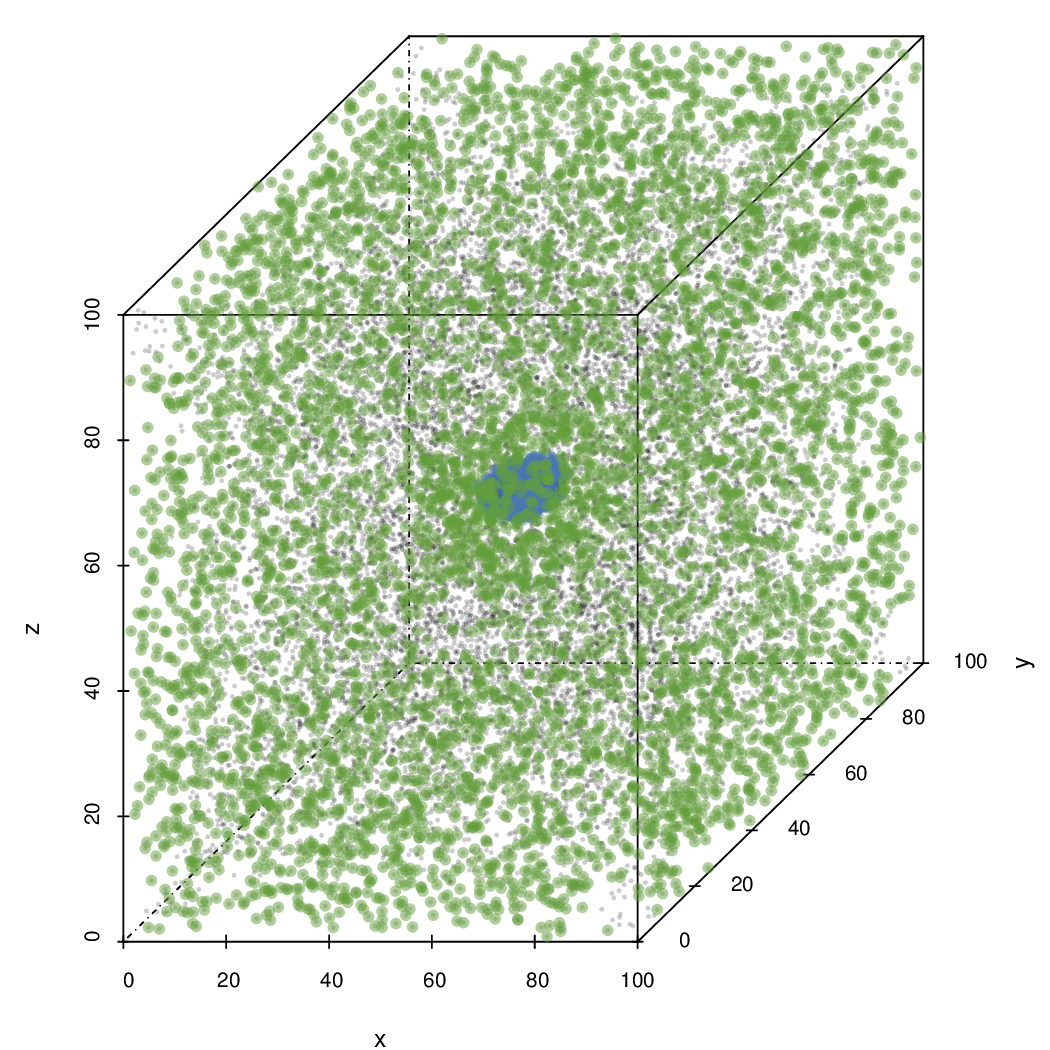
\includegraphics[keepaspectratio=true, width=\textwidth, height=0.23\textheight]{discussion/img/anisotropy_1_60000_anisotropy.png}
			\caption{\anisotropyOne}
			\label{fig:discussion:anisotropy:anisotropy1}
		\end{subfigure}
		\begin{subfigure}{0.23\textwidth}
			\centering
			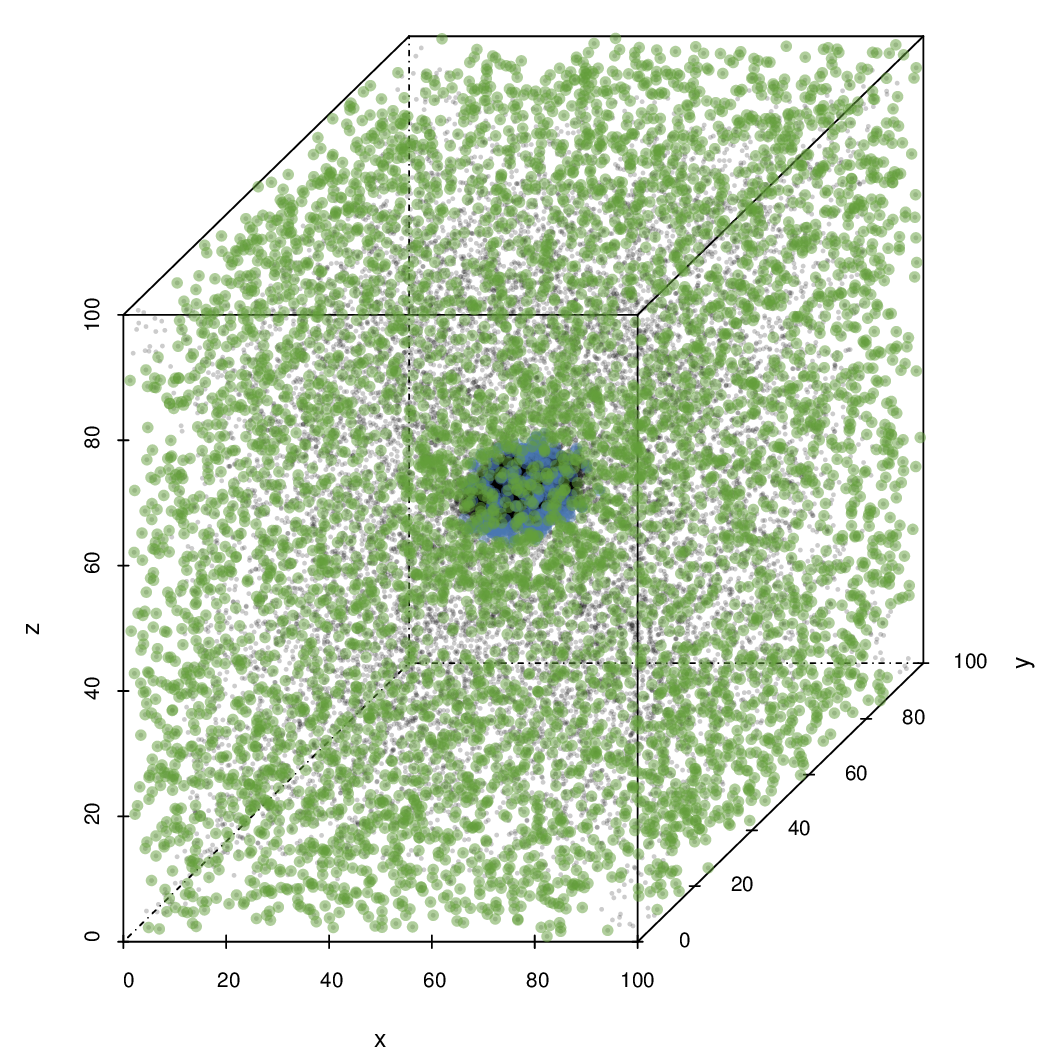
\includegraphics[keepaspectratio=true, width=\textwidth, height=0.23\textheight]{discussion/img/anisotropy_2_60000_anisotropy.png}
			\caption{\anisotropyTwo}
			\label{fig:discussion:anisotropy:anisotropy2}
		\end{subfigure}	
		\caption{Scatter plot of data set \subref{fig:discussion:anisotropy:anisotropy1} \anisotropyOne and \subref{fig:discussion:anisotropy:anisotropy2} \anisotropyTwo, with emphasized the points whose kernels have an anisotropy in the \nth{90} percentile.}
		\label{fig:discussion:anisotropy:anisotropy}
	\end{figure}

% Some conclusion

\todo[inline]{Suggest increasing K: which problems would that solve, discuss experiment with K10}
\todo[inline]{Suggest not always using a shape-adaptive kernel, only if the local neighbourhood has an anistropy that is greater than x. Which problems might that solve?}